\documentclass[11pt]{article}
\usepackage[utf8]{inputenc}
\usepackage[a4paper,width=170mm,top=25mm,bottom=25mm,bindingoffset=6mm]{geometry}
\usepackage[spanish]{babel}
\usepackage[T1]{fontenc}
\usepackage{graphicx}
\usepackage{longtable}
\usepackage{amsmath}
\usepackage{booktabs}
\usepackage{rotating}
\usepackage{amssymb}

\addto\captionsspanish{%
    \def\tablename{Tabla}%
}

\graphicspath{ {figuras/} }

\title{Estudio de convergencia}
\author{}
\date{}


\begin{document}

\maketitle

\subsection{Introducción}

Un estudio de convergencia de malla es una herramienta para evaluar los errores
de discretización espacial de un estudio de CFD y consiste básicamente en:

\begin{enumerate}
    %
    \item Seleccionar un indicador del tamaño de malla $h$.
    %
    \item Elegir un indicador de la convergencia de malla $f$, suele ser la
        variable de estudio.
    %
    \item Seleccionar un coeficiente de refinamiento $r$ y realizar al menos 2
        simulaciones, manteniendo $r$ constante.
    %
    \item Calcular el orden de convergencia de la serie de datos $p$.
    %
    \item Estimar $f_{h=0}$
    %
    \item Calcular el Índice de Convergencia de Malla (GCI por sus siglas en
        inglés).
    %
    \item Comprobar que se está dentro del rango asintótico de convergencia.
    %
\end{enumerate}

El error de discretización surge de aplicar las ecuaciones de gobierno a un
dominio espacial discreto (la malla).
%
A medida que se reduce el tamaño de celda, el resultado del estudio de CFD se
vuelve menos sensible a mayores refinamientos y es esperable que el error de
discretización tienda asintóticamente a cero cuando el tamaño de la malla
tiende a cero.

En la Figura \ref{fig:flujometrias} y la Tabla \ref{tab:casos} se indican los
puntos donde se va a ensayar el puerto de admisión con el fin de obtener el
valor de caudal másico o volumétrico que fluja por el puerto en distintas
posiciones del rotor y a distintas velocidades de rotación.
%
Dada la cantidad de flujometrías a realizar se opta por realizar el estudio de
convergencia solo en algunos de los casos, los cuales serán utilizados como
referencia e indicarán el nivel mínimo de refinamiento mínimo necesario a
utilizar para todos los casos.

% Se utilizará el mismo paso tempral en todos los refinamientos.

\begin{figure}
    \centering
    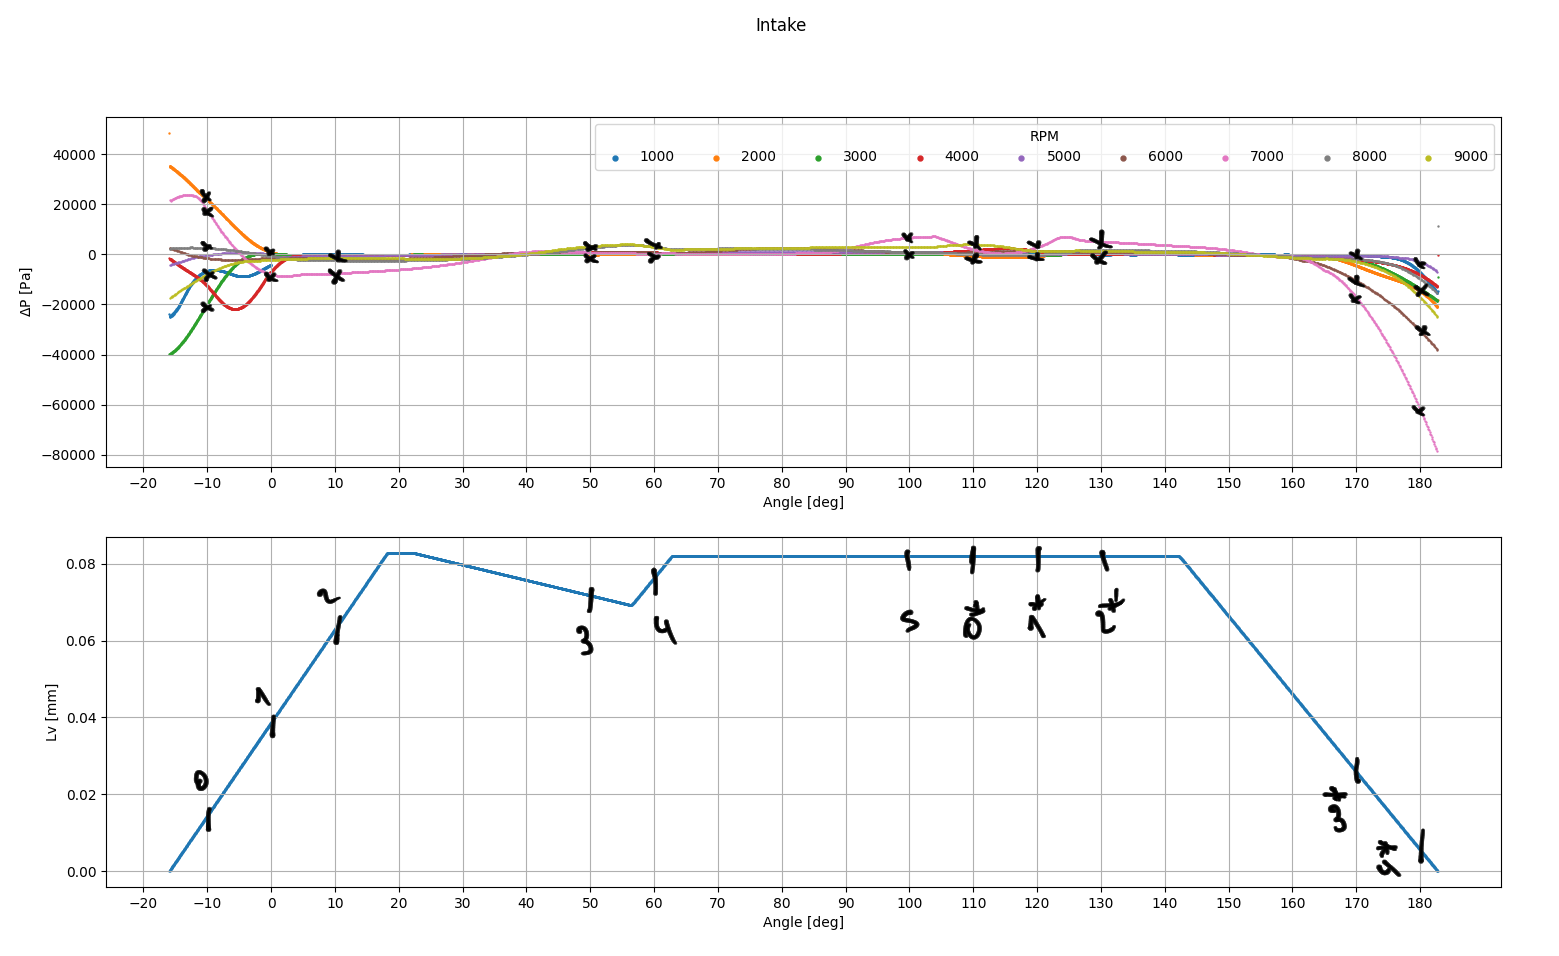
\includegraphics[width=1\textwidth]{flujometrias_admision.png}
    \caption{Flujometrías para el puerto de admisión}
    \label{fig:flujometrias}
\end{figure}

\begin{table}
    \centering
    \begin{tabular}{rcc} \toprule
        Caso & Ángulos & Velocidades (rpm) \\ \midrule
        0 & -10, 110 & 1000, 2000, 3000, 7000, 8000\\
        1 & 0, 120 & 2000, 7000\\
        2 & 10, 130 & 2000, 7000\\
        3 & 50, 170 & 3000, 7000, 9000\\
        4 & 60, 180 & 3000, 5000, 6000, 7000\\
        5 & 95 & 1000, 7000\\ \bottomrule
    \end{tabular}
    \caption{Flujometrías para el puerto de admisión}
    \label{tab:casos}
\end{table}

Hay que distinguir en entre los refinamientos necesarios de flujometrías en
régimen compresible e incompresible, los casos a tomar como referencia son el
0, 4 y 5.

\subsubsection{Selección de $h$, $r$ y $f$}
%
El procedimiento para generar la malla consiste en realizar un primer mallado
con la utilidad \emph{blockMesh} la cual es un punto de partida de
\emph{snappyHexMesh}.
%
Se busca que la malla creada por \emph{blockMesh} este compuesta por celdas
cúbicas, como se ilustra en la Figura \ref{fig:celdas_bm} el lado de estas
celdas es el que se toma como indicador del tamaño de malla $h$.
%
El coeficiente de refinamiento es el cociente entre el tamaño $h$ de dos pasos
de refinamiento, como se indica en la ecuación \ref{eq:r}, el mismo se toma
igual a 1.5 y se mantiene constante para todos los refinamientos.
%
Se realizarán refinamientos con mallas de $11.25mm \rightarrow 7.5mm
\rightarrow 5mm$.

\begin{equation}
    \label{eq:r}
    r = \frac{h_{i+1}}{h_{i}} = 1.5
\end{equation}


\begin{figure}
    \centering
    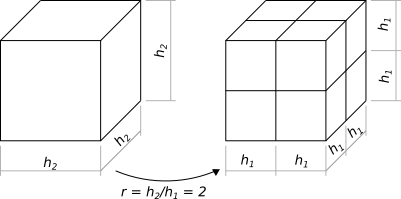
\includegraphics{celdas_block_mesh.png}
    \caption{Refinamiento con $r=2$}\label{fig:celdas_bm}
\end{figure}

Para verificar la convergencia de malla se utiliza el flujo másico a través
de las superficies definidas como entrada/salida de cámaras.
%
En la figura \ref{fig:parches} se indican las superficies por las cuales hay
flujo másico, siempre que haya solape de cámaras, la cámara que esté a la
izquierda será llamada cámara 0 y la que esté a derecha cámara 1.
%
La superficie que indica la conexión entre el puerto y el resto de los conductos
de intercambio de gases se denominará puerto.


En caso de flujo presente un $Ma < 0.3$, el \emph{solver} a utilizar devuelve
el flujo volumétrico, por lo que se usa este como indicador en lugar del flujo
másico.

\begin{figure}
    \centering
    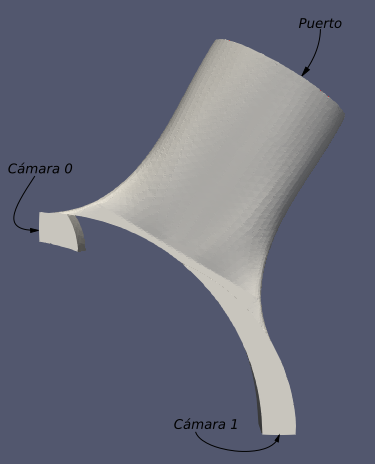
\includegraphics[width=0.4\textwidth]{nombres-parches.png}
    \caption{Vista superior del volumen de control}\label{fig:parches}
\end{figure}

\subsubsection{Orden de convergencia}
%
El orden de convergencia $p$ indica que tan rápido se acerca una secuencia a un
límite.
%
Una secuencia ${x_n}$ que converge a $x^*$ tiene orden de convergencia $p \ge
1$ y constante asintótica de error $\mu$.

\begin{equation}
    \lim_{n\rightarrow \infty} \frac{|x_{n+1} - x^*|} {|x_{n} - x^*|^p} = \mu
\end{equation}

El orden de convergencia se puede obtener de comparando el comportamiento del
error, definido como la diferencia ente la solución exacta o del continuo y la
discreta.

\begin{equation}
    E = f(h) - f_{exacta} = Ch^p + \xi
    \label{eq:1}
\end{equation}

Dónde $C$ es una constante, $h$ es una medida del nivel de refinamiento de la
malla, $p$ es el orden de convergencia y $\xi$ son términos de orden superior.
%
Despreciando los términos de orden superior $\xi$ y tomando logaritmo a ambos
lados, se puede expresar la ecuación \ref{eq:1} como:

\begin{equation}
    \log(E) = \log(C) + p \cdot \log(h)
\end{equation}

De esta forma $p$ es la pendiente de la curva de $\log(E)=f(\log(h))$ y
conociendo al menos 3 puntos puede calcular $p$ como:

\begin{equation}
p = \ln \left( \frac{ f_3 - f_2 } { f_2 - f_1 } \right) / \ln(r)
\label{eq:ord-conv}
\end{equation}

\subsubsection{Resultado ''exacto``}
%
El resultado de una simulación numérica se puede expresar de forma general
como:

\begin{equation} \label{eq:expansion}
    f = f_{h=0} + g_1 h + g_2 h^2 + g_3 h^3 + ...
\end{equation}

Dónde $h$ es el tamaño de la malla y $g_1$, $g_2$ y $g_3$ son funciones
independientes $h$, la cantidad $f$ es considerada de segundo orden si $g1 =
0$.
%
El valor de $f_{h=0}$ es el resultado que tendría la simulación con una malla
infinitamente fina, $h \rightarrow 0$.

\subsection{Índice de convergencia de malla}
%
El índice de convergencia de malla o GCI por sus siglas en inglés es una forma
de reportar los resultados de convergencia de malla, es un indicador de qué tan
lejos se encuentran los resultados obtenidos del resultado numérico exacto
($f_{h=0}$) y surge de la siguiente ecuación:

\begin{equation} \label{eq:gci}
GCI_{i \rightarrow j} = \frac{F_S |\epsilon|}{r^p - 1}
\end{equation}

Dónde:
\begin{description}
    \item[$F_S$] es un factor de seguridad, se toma 1.25.
    \item[$\epsilon$] es el error relativo $\epsilon = (f_i - f_j) / f_j$
    \item[$r$] es el factor de refinamiento $r = h_i/h_j$
    \item[$p$] es el orden de convergencia relativo a los pasos i, j
\end{description}

De este modo, si para un nivel de refinamiento $h_i$ la simulación da como
resultado un valor $x_i$ con $GCI_i$ dado, se puede decir que el resultado
de la simulación es $x_i \pm GCI_i \cdot 100$.
%
Se tomará como GCI aceptable o banda de error un valor cercano a 5\%.

\section{Resultados}

Para determinar el tipo de \emph{solver} a utilizar se hace una primer corrida
de cada caso asumiendo que el flujo se puede asumir como incompresible, es
decir, que el número de Mach máximo del caso convergido va a ser menor a 0.3.
%
Estos resultados no son definitivos en cuanto al \emph{solver} a utilizar,
puede suceder que a medida que refine un caso el $Ma$ aumente, en cuyo caso
se deberá evaluar si es necesario revisar la hipótesis de flujo incompresible.

% ESe dice que el caso converge cuando el flujo másico a través de cualquiera de
% las entradas/salidas del dominio se estabiliza.

\begin{table}
    \centering
    \begin{tabular}{rll}\toprule
        Caso & Velocidad [RPM] & $Ma_{max}$ \\ \midrule
        0 & 1000 & 0.29 \\
        0 & 2000 & 0.65 \\
        0 & 3000 & 0.49 \\
        0 & 7000 & 0.65 \\
        0 & 8000 & 0.23 \\
        1 & 2000 & 0.14 \\
        1 & 7000 & 0.4 \\
        2 & 2000 & 0.1 \\
        2 & 7000 & 0.43 \\
        3 & 3000 & 0.16 \\
        3 & 7000 & 0.37 \\
        3 & 9000 & 0.24 \\
        4 & 3000 & 0.35 \\
        4 & 5000 & 0.38 \\
        4 & 6000 & 0.49 \\
        4 & 7000 & 0.63 \\
        5 & 1000 & 0.01 \\
        5 & 7000 & 0.45 \\ \bottomrule
    \end{tabular}
    \caption{Números de Mach}
    \label{tab:mach}
\end{table}

\subsection{Caso 0 - 1000rpm}

El caso simulado tiene solape de cámaras, una a $-10^{\circ}$ y otra a
$110^{\circ}$, con el motor girando a 1000 RPM.
%
El flujo se modela como incompresible\footnote{Ver Tabla \ref{tab:mach}}, la
geometría del caso y la ubicación de los parches correspondeintes a la cámara
0, 1 y a la "boca" del puerto.

\begin{figure}
    \centering
    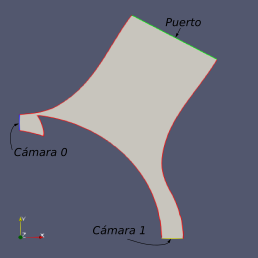
\includegraphics{caso0.png}
    \caption{Geometría a modelar}
    \label{fig:caso0}
\end{figure}

\begin{table}
    \centering
    \begin{tabular}{rll}\toprule
        Parámetro & Valor \\ \midrule
        $\theta_0\ [^{\circ}]$ & 590 \\
        $\theta_1\ [^{\circ}]$ & 110 \\
        $\epsilon_{est}$ & 195.467 \\
        $\gamma_{est}$ & 1.309 \\
        $\kappa_{est}$ & 1.364471 \\
        $\nu_{est}$ & 4.3e-05 \\
        $p_0 [Pa]$ & 107355.2 \\
        $p_1 [Pa]$ & 100867.47 \\
        $\overline{p} [Pa]$ & 104111.33 \\
        $\overline{p_{puerto}} [Pa]$ & 100780.23 \\
        $\overline{\rho} [kg/m^3]$ & 0.643938 \\
        $\overline{T} [K]$ & 589.89 \\ \bottomrule
    \end{tabular}
    \caption{Valores iniciales}
    \label{tab:caso0_ci}
\end{table}


En la tabla \ref{tab:res_caso0}se muestran los resultados de 3 pasos de
refinamiento. TENGO QUE REHACER TODOS EN REGIMEN COMPRESIBLE

\begin{table}
    \centering
    \begin{tabular}{rccccc}\toprule
        h [mm] & $h_{norm}$ & $N^{\circ}$ celdas & $Ma$ & $\dot{V_{0}}\ [m^3/s] $ & $\dot{V_{1}}\ [m^3/s]$ \\ \midrule
        5      & 1.0        & 167900             & 0.36 & -0.006312     & -0.012329 \\
        10     & 2.0        & 52210              & 0.33 & -0.006455     & -0.011692 \\
        20     & 4.0        & 20795              & 0.29 & -0.006668     & -0.011652 \\ \bottomrule
    \end{tabular}
    \caption{Flujos volumétricos para ambas cámaras}
    \label{tab:res_caso0}
\end{table}

Con estos datos se puede calcular el orden de convergncia y el resultado
extrapolado a $h=0$.

\begin{table}
    \centering
    \begin{tabular}{rcc}\toprule
        Parámetro & Cámara 0  & Cámara 1  \\ \midrule
        p         &  0.565833 & -3.967099 \\
        $f_{h=0}$ & -0.006013 & -0.011649 \\ \bottomrule
    \end{tabular}
    \caption{Orden de convergencia y resultado exacto}
    \label{tab:res1_caso0}
\end{table}

Y con el orden de convegencia se pueden calcular los valores de GCI.

\begin{table}
    \centering
    \begin{tabular}{rccc}\toprule
        Paso              & $r$ & $GCI_0(\%)$ & $GCI_1(\%)$ \\ \midrule
        1 $\rightarrow$ 2 & 2   & -5.923628   & 6.895404 \\
        2 $\rightarrow$ 3 & 2   & -8.573288   & 0.464910 \\ \bottomrule
    \end{tabular}
    \caption{GCI}
    \label{tab:gci_caso_0}
\end{table}

Con estos resultados se verifica que se esté en rango de convergencia
asintótica, como se indica en la Tabla \ref{tab:rac_caso_0}, los flujos
másicos de ambas cámaras se encuentran en rango de convergencia asintótica.

\begin{table}
    \centering
    \begin{tabular}{rccc}\toprule
        Rango               & $rac_0$  & $rac_1$ \\ \midrule
        12 $\rightarrow$ 23 & 1.022758 & 0.948364 \\ \bottomrule
    \end{tabular}
    \caption{Verificación de convergencia}
    \label{tab:rac_caso_0}
\end{table}


\subsection{Caso 0 - 7000 rpm}

\subsection{Caso 4 - 7000 rpm}

\subsection{Caso 5 - 1000rpm}

El caso simulado tiene una sola cámara a $100^{\circ}$ del ciclo, con el motor
girando a 1000 RPM.
%
El flujo se modela como incompresible\footnote{Ver Tabla \ref{tab:mach}}, la
geometría del caso y la ubicación de los parches correspondeintes a la cámara
0, 1 y a la "boca" del puerto.

\begin{figure}
    \centering
    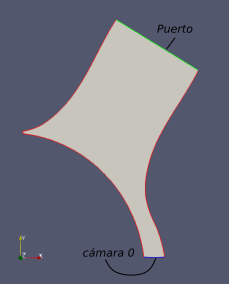
\includegraphics{caso5.png}
    \caption{Geometría a modelar}
    \label{fig:caso5}
\end{figure}

\begin{table}
    \centering
    \begin{tabular}{rll}\toprule
        Parámetro & Valor \\ \midrule
        $\theta_0\ [^{\circ}]$ & 100 \\
        $\epsilon_{est}$ & 25.271765 \\
        $\gamma_{est}$ & 1.329 \\
        $\kappa_{est}$ & 0.348878 \\
        $\nu_{est}$ & 2.9e-05 \\
        $\overline{p} [Pa]$ & 103732.67 \\
        $\overline{p_{puerto}} [Pa]$ & 103773.09 \\
        $\overline{\rho} [kg/m^3]$ & 0.797554 \\
        $\overline{T} [K]$ & 453.18 \\ \bottomrule
    \end{tabular}
    \caption{Valores iniciales}
    \label{tab:caso5_ci}
\end{table}

En la tabla \ref{tab:res_caso5} se muestran los resultados de 3 pasos de
refinamiento.

\begin{table}[h]
    \centering
    \begin{tabular}{rcccc}\toprule
        h [mm] & $h_{norm}$ & $N^{\circ}$ celdas & $Ma$ & $\dot{V}\ [m^3/s]$ \\ \midrule
        5      & 1.0        & 167900             & 0.36 & -0.006312 \\
        10     & 2.0        & 52210              & 0.33 & -0.006455 \\
        20     & 4.0        & 20795              & 0.29 & -0.006668 \\ \bottomrule
    \end{tabular}
    \caption{Flujos volumétricos para ambas cámaras}
    \label{tab:res_caso5}
\end{table}

Con estos datos se puede calcular el orden de convergncia y el resultado
extrapolado a $h=0$.

\begin{table}[h]
    \centering
    \begin{tabular}{rc}\toprule
        Parámetro & Cámara 0  \\ \midrule
        p         &  0.565833 \\
        $f_{h=0}$ & -0.006013 \\ \bottomrule
    \end{tabular}
    \caption{Orden de convergencia y resultado exacto}
    \label{tab:res1_caso5}
\end{table}

Y con el orden de convegencia se pueden calcular los valores de GCI.

\begin{table}
    \centering
    \begin{tabular}{rcc}\toprule
        Paso              & $r$ & $GCI_0(\%)$ \\ \midrule
        1 $\rightarrow$ 2 & 2   & -5.923628   \\
        2 $\rightarrow$ 3 & 2   & -8.573288   \\ \bottomrule
    \end{tabular}
    \caption{GCI}
    \label{tab:gci_caso_5}
\end{table}

Con estos resultados se verifica que se esté en rango de convergencia
asintótica, como se indica en la Tabla \ref{tab:rac_caso_5}, los flujos
másicos de ambas cámaras se encuentran en rango de convergencia asintótica.

\begin{table}
    \centering
    \begin{tabular}{rccc}\toprule
        Rango               & $rac_0$  \\ \midrule
        12 $\rightarrow$ 23 & 1.022758 \\ \bottomrule
    \end{tabular}
    \caption{Verificación de convergencia}
    \label{tab:rac_caso_5}
\end{table}

\subsection{Caso 5 - 7000rpm}

\subsection{Resultado final}

\end{document}
